\providecommand{\main}{..}

\documentclass[/home/francois/latex/report/main.tex]{subfiles}

\begin{document}

\chapter{Method}
\label{chapter:method}

This chapter presents the inertial parameters estimation approach starting with the signal pre-processing, followed by the robot manipulator calibration and the objective function computation.

The overall idea is to compute the objective function matrices so as to estimate the parameters with a \ac{LS} method. A crucial step is the upstream calibration of the tool and gripper parameters. They are non obvious and non documented properties that have to be estimated before running the overall process. An overview of the framework of the inertial parameters estimation is depicted in the Figure \ref{fig:method:overall}.

\begin{figure}[H]
  \centering
  \includegraphics[scale=0.7]{\main/figures/olinpe.pdf}
  \caption{Overview of the payload inertial parameters estimation approach. The calibration process is an upstream step that is done whenever the gripper tool is modified. Image from  the author.}
  \label{fig:method:overall}
\end{figure}

\section{Signal Pre-processing}
\label{section:pre-pro}

In the chaper \ref{chapter:background}, two models of the \{item\} and \{tool\} systems have been developed. The purpose is to compute the matrices of the equation and then use one or another optimization process. The matrices $A$ and $B$ (respectively $A'$ and $B'$) are computed out of the \ac{FT} sensor measurement and the position and orientation of the \ac{TCP}. One point must be made: signals cannot be merely input in the optimization procedures. Both \ac{FT} measurements and simple method for derivation leads to noisy signals. Consequently, measured signals have to be pre-processed.

\subsection{\textsc{Euler}'s angles continuity filter}

The input orientation of the \ac{TCP} is expressed as \ac{RPY} \textsc{Euler}'s angles. Thus, they are computed in a range of $[-\pi, \pi]$. Approaching to the interval limit (cf. \ref{section:results:pre-processing}), the signal jumps from positive to negative $\pi$. In addition, the representation by \textsc{Euler}'s angles has no unicity because it depends on the order of axes (anisotropy). When deriving the angular speed and angular acceleration, the outcome is consequently unsatisfying. To tackle that unicity issue, the great properties of quaternion conversion are applied to the set of angles. Subsenquently, the \ac{RPY} angles are filtered with a continuity algorithm (cf. Algorithm \ref{alg:method:continuity}).

The quaternion filter consists in three steps:

\begin{itemize}
  \item convert the \textsc{Euler}'s angles to quaternion,
  \item compute the rotation matrix out of the quaternion vector,
  \item convert the rotation matrix to a \ac{RPY} set of angle.
\end{itemize}

\begin{algorithm}
\caption{Ensure continuity of an \textsc{Euler}'s angles signal \label{alg:method:continuity}}
\begin{algorithmic}
\FOR{\texttt{orientation} in \texttt{signal}}
 \FOR{\texttt{angle} in \texttt{orientation}}
  \STATE \texttt{previous}  $\leftarrow$ \texttt{current}
  \STATE \texttt{current}  $\leftarrow$ \texttt{angle}
  \IF{$\text{\texttt{current}} \times \text{\texttt{previous}} < 0$}
   \IF{$\text{\texttt{current}} - \text{\texttt{previous}} > 0$}
    \STATE $\text{\texttt{angle}} \leftarrow \text{\texttt{current}} - 2 \pi$
   \ELSE
    \STATE $\text{\texttt{angle}} \leftarrow \text{\texttt{current}} + 2 \pi$
   \ENDIF
  \ENDIF
 \ENDFOR
\ENDFOR
\end{algorithmic}
\end{algorithm}

\subsection{\textsc{Savitzky–Golay} filter}

Therefore, it is needed to derived the linear and angular velocity and the linear and angular speed from the \ac{TCP} pose. First tests conducted with simple derivation method using $f'(t) \approx  [f(t+\delta) - f(t)] / \delta$ does not provide good results (cf. comparison in \ref{section:results:pre-processing}). The noise induced in the \ac{TCP} pose measurement generates spikes in the derivated signal. One approach is to use \textsc{Savitzky–Golay} filter to guatantee smooth derivated signals.

The method was created in 1964 by A. \textsc{Savitzky} M. J. E. \textsc{Golay} \cite{Savitzky1964} in their seminal article. The smoothing of a signal or its derivative is achieved with a convolution process. Sub-sets of adjacent data points are fitted to a low-degree polynomial by the method of linear \ac{LS} (cf. \ref{fig:method:savit}). Convoluation coefficients are then use to give estimates of the smoothed signal, (or derivatives of the smoothed signal) at the central point of each sub-set.

\begin{figure}[H]
  \centering
  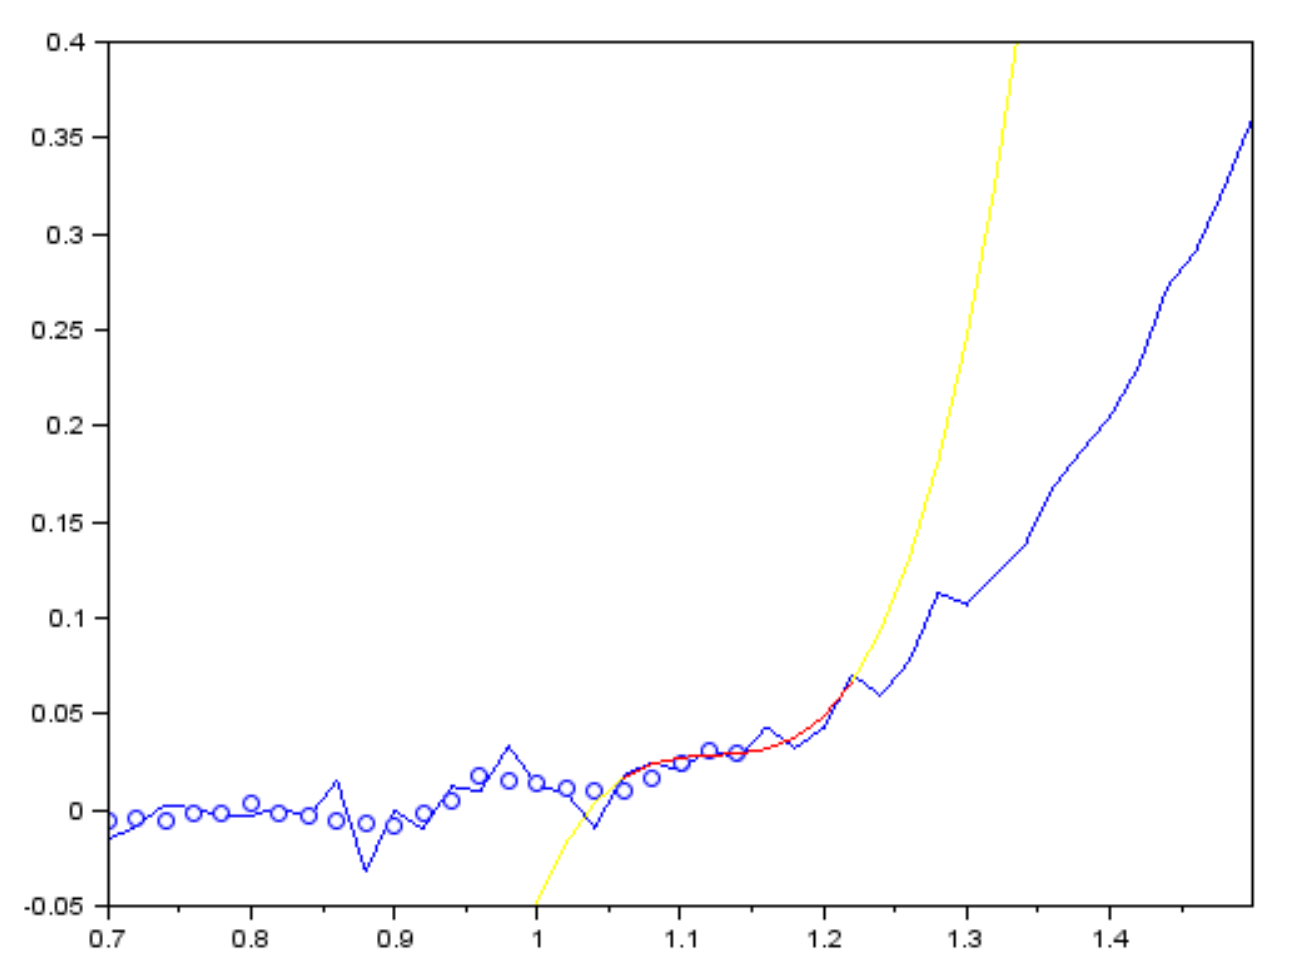
\includegraphics[scale=0.25]{\main/figures/savitzky-golay-filter.png}
  \caption{Smoothing of noisy data by the \textsc{Savitzky–Golay} method ($3^{rd}$ degree polynomial, 9 points wide sliding window). Blue curve: raw data; blue circle: point after smoothing; yellow curve: polynomial used to determine the current point; red curve: polynomial restricted to the sliding window around the current point. Image from \cite{Cdang2013}.}
  \label{fig:method:savit}
\end{figure}

\subsection{Low-pass filter}

As mentioned above, the \ac{FT} signal is slightly noisy. As the frequency of the noise is relatively high, it is considered to use a low-pass filter. The choice fell on the \textsc{Butterworth} filter (cf. \cite{filter1923}), a signal processing filter which is having a flat frequency response in the passband can be termed as Butterworth filter and is also called as a maximally flat magnitude filter (cf. \ref{fig:method:butter}).

Besides, this low-pass filter is applied twice, once forward and once backwards. The combined filter has zero phase and a filter order twice that of the original \cite{SciPy2019}.

\begin{figure}[H]
  \centering
  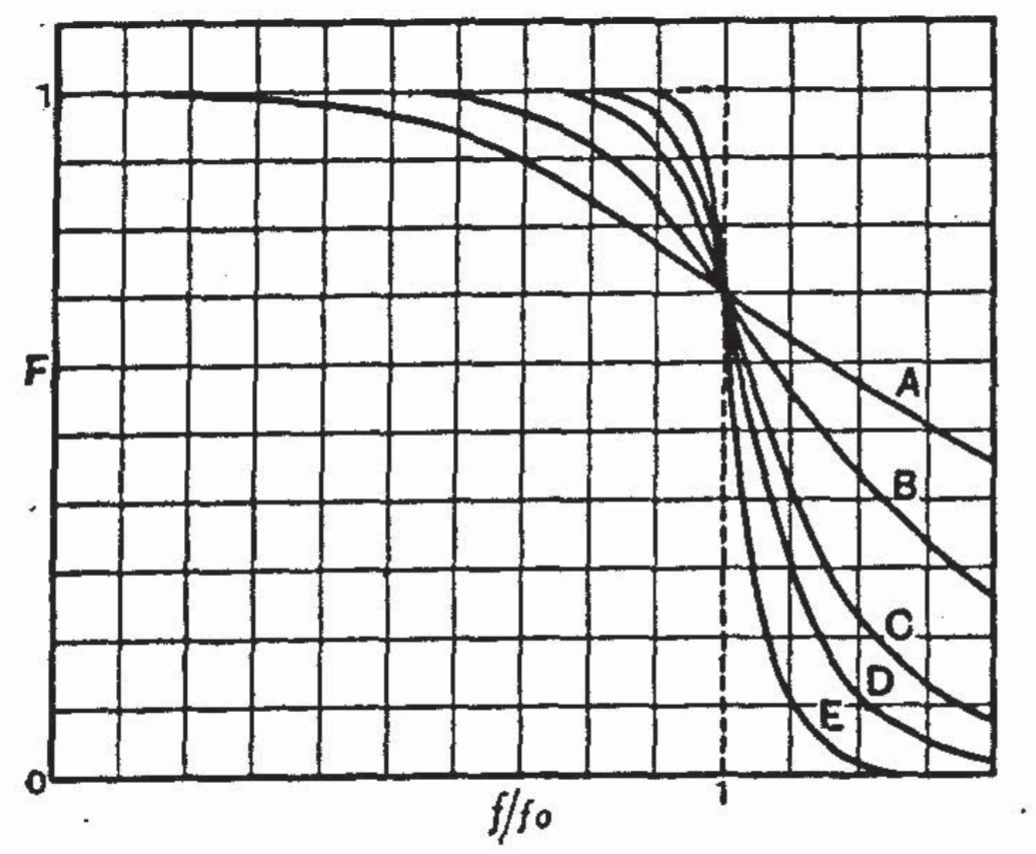
\includegraphics[scale=0.25]{\main/figures/butter.png}
  \caption{Frequency response plot from different order \textsc{Butterworth} filter. Image from the original article  \cite{filter1923}.}
  \label{fig:method:butter}
\end{figure}

\section{Calibration of the robot manipulator}

In the section \ref{section:pre-pro}, it was mentioned that the matrices $A$ and $B$ (respectively $A'$ and $B'$) are computed out of signal measurements. One can notice, that several robot manipulator and gripper constants are necessary to completely compute the matrices. In particular, the mass of the tool $m_1$, its center of mass $c_1$, its tensor of inertia $I_1$ and the suction cup properties: the spring coefficient $k$, damping ratio $\lambda$ are needed.

\subsection{Tool inertial parameters}

The tool inertial parameters ($\varphi_1$) can be estimated by using the rigid model defined in section \ref{section:background:rigid}. Axes of inertia of the tool can be \textit{excited} by moving the tool in different directions, at different linear and rotational speeds. \textsc{Kubus} \textit{et al.} \cite{Kubus2008} advice to design sinusoidal excitation trajectories in the joint space. They can be optimized by minimizing the sensitivity of $\varphi_1$ to errors in $A$ (cf. equation \ref{background:eq:inertia_estimation}). The project does not focus on the design of such trajectories. Consequently, the motion is a simple trapezoidal speed profile in multiple directions and about multiple axes of rotation (cf. \ref{fig:method:trajectory}).

\begin{figure}[H]
\centering
\begin{subfigure}{\textwidth}
\centering
\includegraphics[scale=0.2]{\main/figures/load_free_position.pdf}
\caption{Position of the \ac{TCP} over time}
\label{fig:method:position}
\end{subfigure}
\begin{subfigure}{\textwidth}
\centering
\includegraphics[scale=0.2]{\main/figures/load_free_orientation.pdf}
\caption{Orientation of the \ac{TCP} over time}
\label{fig:method:orientation}
\end{subfigure}
\caption{Trajectory for the estimation of the tool inertial parameters and suction properties. The \ac{TCP} is excited in different directions and about different axes of rotation to embed as much mechanical properties as possible in the measurements. Images from the author.}
\label{fig:method:trajectory}
\end{figure}

\subsection{Spring constant and damper coefficient estimation}

The \ac{RMSD} model strongly depends on a good estimation of the spring constant and damper coefficient. There is a broad range of suction cups of different diameters, lengths, materials –and colors (cf. \ref{fig:method:suction-cups}). Therefore there is as many combinations of spring and damper constants.

\begin{figure}[H]
  \centering
  \includegraphics[scale=0.4]{\main/figures/suction_cup.jpg}
  \caption{A huge diversity of suction cups. Image from \cite{Piab2020}.}
  \label{fig:method:suction-cups}
\end{figure}

The idea is to make use of the equations of the \ac{RMSD} system to extract the constants $k$ and $\lambda$. For that purpose, a plane system is considered, with a limited \ac{DoF}. The \textsc{Newton-Euler} equations are derived for each subsystem \{item\} and \{tool\} to compute the orientation (cf. equation \ref{eq:method:force_2d}) of the item about the tool as a function of the force measured by the \ac{FT} sensor and the inertial parameters of the assembly (cf. details in the Appendix \ref{appendix:plane-rmsd}).

\begin{equation}
  \label{eq:method:force_2d}
  \overrightarrow{f}
  =
  \begin{pmatrix}
  0 \\
  m_1 a_y + m_2 [a_y + c (\dot{\theta}^2 \theta - \ddot{\theta})] \\
  m_1 (a_z + g) + m_2 [a_z + g + c (\dot{\theta}^2 + \ddot{\theta} \theta)]
  \end{pmatrix}
\end{equation}

Therefore, the vacuum cup is calibrated with a standard object of known mass $m_2$, center of mass $c_2$ and inertia tensor $I_2$. This object can be a solid cuboid of aluminium which dimensions and mass are known. The robot manipulator and the suction cup are then \textit{excited} with a similar flat trajectory than the one depicted in the figure \ref{fig:method:trajectory}. One can notice here that the system is very similar to an harmonic pendulum. Hence, the transient of the system should provide sufficient information to estimate the two parameters.

From the torque \ac{FPD} applied to the \{item\}, an \ac{ODE} (cf. equation \ref{eq:method:torque_2d}) is obtained. As, the angle $\theta$ can be computed, the constants are merely estimated with a \ac{LS} algorithm.

\begin{equation}
  \label{eq:method:torque_2d}
 \ddot{\theta} + \frac{\lambda}{I_{2xx}} \dot{\theta} + \frac{k + m_2 c (a_z + g)}{I_{2xx}} \theta = - \frac{m_2 c}{I_{2xx}} a_y
\end{equation}

It is rather complicated to have an accurate feedback on the estimation of such properties. There is no abacus from suction cup supplier to validate the result. Thus, the validation method consists of comparing the estimated force and torque signals with the measured \ac{FT} ones with a different standard item.

\section{Inertial parameters estimation strategy}



\end{document}
